\documentclass[a4paper]{article}

\usepackage[english]{babel}
\usepackage[utf8]{inputenc}
\usepackage{amsmath}
\usepackage{amssymb}
\usepackage{centernot}
\usepackage{graphicx}
\usepackage[colorinlistoftodos]{todonotes}
\usepackage{listings}
\usepackage{color}
\usepackage{booktabs}
\usepackage{hyperref}
\usepackage{tcolorbox}
\hypersetup{
 colorlinks=true,
 linkcolor=blue,
 urlcolor=blue
}


\lstset{
	breaklines=true,
	basicstyle=\footnotesize,
	mathescape=false,
	frame=single,
	keepspaces=true,
	keywordstyle=\color{blue}
}


\lstdefinestyle{Bash}
{language=bash,
keywordstyle=\color{blue},
basicstyle=\ttfamily,
morekeywords={peter@kbpet},
alsoletter={:~$},
morekeywords=[2]{peter@kbpet:},
keywordstyle=[2]{\color{red}},
literate={\$}{{\textcolor{red}{\$}}}1 
         {:}{{\textcolor{red}{:}}}1
         {~}{{\textcolor{red}{\textasciitilde}}}1,
}



\usepackage{titlesec}

\setcounter{secnumdepth}{4}

\titleformat{\paragraph}
{\normalfont\normalsize\bfseries}{\theparagraph}{1em}{}
\titlespacing*{\paragraph}
{0pt}{3.25ex plus 1ex minus .2ex}{1.5ex plus .2ex}


\newcommand*{\squiggly}{\rightsquigarrow}



\title{Notes on Phosphor}
\author{Jos\'e Cambronero}







\begin{document}
\maketitle
\begin{abstract}
This document contains my personal set of notes for building and running examples with Jonathan Bell's
Phosphor\cite{bell2014phosphor}. This should be viewed as a beginners guide (as I am writing it
as I learn to use the tool myself.) Any errors or omissions here are my own.
\end{abstract}

\section{Installation/Building}
\label{install}
We begin by cloning the \href{https://github.com/Programming-Systems-Lab/phosphor}{github repository}
for the project.

\begin{lstlisting}
$ git clone git@github.com:Programming-Systems-Lab/phosphor.git
\end{lstlisting}

Phosphor is a \href{https://maven.apache.org/}{maven} project, so to build you can call
\verb|mvn package|. As per the documentation
Phosphor has been built and tested with both versions 7/8 of Oracle's Hotspot JVM and
OpenJDK's IcedTea JVM. If you run into issues with your java version, I suggest installing
\href{http://www.jenv.be/}{jenv}, which allows you to manage multiple versions of the JVM on your
machine cleanly and transparently.

\begin{lstlisting}
$ jenv local 1.8.0.66
$ mvn package
\end{lstlisting}

You should obtain a message similar to the one in Figure~\ref{fig:phosphor-build} if your build was succesful

\begin{figure}
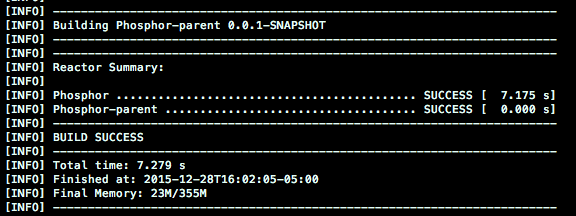
\includegraphics[width=\textwidth]{figures/phosphor-build}
\caption{Succesful build message}
\label{fig:phosphor-build}
\end{figure}

Now, we need to instrument our JRE before we can run any of our examples. This can be done
as follows

\begin{lstlisting}
$ cd target/
$ java -jar Phosphor-0.0.2-SNAPSHOT.jar \
 /Library/Java/JavaVirtualMachines/jdk1.8.0_66.jdk/Contents/Home/jre/ jre-inst/
\end{lstlisting}

This has created an instrumented JRE suitable for data flow tracking and integer
tags combined with $OR$.

The only thing left to do is make sure we change permissions for all binaries in
the instrumented JRE.

\begin{lstlisting}
$ chmod +x jre-inst/bin/*
\end{lstlisting}

\section{Testing}
In order to verify that your build works, you can run the \verb|mvn verify| command, as explained in the documentation.
You should expect this to take a bit, as it generates different instrumented JREs and tests them.
% Ran into issues with ReflectionImplicitITCase with 1.7, switched to 1.8, emailed Jonathan
% to see if this is expected or not.



\section{Usage}
\subsection{Automatic}
TODO: this remains to be experimented with
TODO: taintSinks/taintSources usage


\subsection{Data flow}
In this section we will focus on examples that track taint from data flow operations, usually referred to as 
explicit flows\cite{denning1976lattice}. Assume $x$ is tainted, an operation such as $y = x * 2$ taints $y$.

\subsubsection{Integer taint tags}
Phosphor allows users to track taint tags represented as integers (allowing up to 32 different taint
tags), or objects, which allows up to $2^{32}$ tags. In this section we focus on integer taint tags.
Consequently, we also focus our API attention to \verb|edu.columbia.cs.psl.phosphor.runtime.Tainter|.
In it, we will primarily use 2 methods, as noted in the
original documentantion: \verb|taintedX|, which allows us to mark a primitive source as tainted, and
\verb|getTaint| which we can use to check for taint.

We show a series of simple examples using this across different datatypes. Note that the types 
can be easily replaced. Note that for each example we only show part of the relevant code,
the interested reader can check the source code associated with this guide
in \verb|com.josecambronero.IntegerTagExamples|.

\paragraph{Simple binary operation}
In this simple example, we create a source for the taint (variable $x$), and want to check
if there is taint flow from our source to a sink (variable $y$). In this case, $y$ is the result
of an assignment operation involving $x$, and thus should be tainted.

We can use \verb|Tainter.taintedInt| to taint $x$, and \verb|Tainter.getTaint| to check the taint
tag for $y$.

\begin{lstlisting}
// source
int x = 0;
// sink
int y = 0;
// primitive and taint tag
x = Tainter.taintedInt(x, 1);
y = x * 3;
// check sink for taint
assert (Tainter.getTaint(y) != 0);
\end{lstlisting}



\paragraph{Nullifying taint}
Note that the taint for a sink can change throughout the program. For example,
if we define $y$ in terms of a tainted $x$ and then redefine $y$ as a constant, the final $y$
is not tainted. The excerpt from \verb|IntegerTagExamples.testExample2|  below
shows this behavior.

\begin{lstlisting}
// source
int x = 0;
// sink
int y = 0;
x = Tainter.taintedInt(x, 1);
// tainted
y = x * 3;
assert (Tainter.getTaint(y) != 0);
// not tainted, as zero returns constant (not function of x)
y = zero(x);
assert (Tainter.getTaint(y) == 0);
\end{lstlisting}


\paragraph{Arithmetic identity}
Note that some arithmetic identities, which would allow a human to easily determine that no
taint exists, as the result is always constant, will yield a tainted tag with taint analysis.
So for example, in the excerpt below $y$ is tainted despite the fact that it assigned 0, regardles
of the tainted value of $x$.

\begin{lstlisting}
// source
int x = 1;
x = Tainter.taintedInt(x, 1);
// sink
int y = 0;
y = 2 * x - (x + x);
assert (Tainter.getTaint(y) != 0);
\end{lstlisting}

\paragraph{Tracking Source of Taint}
Phosphor allows the user to track the source of the taint in a sink by exploring the values
of the taint tag. A similar functionality is available for the MultiTainter by exploring
the dependencies of the tag.

In the example below, we can see that $y$ has taint stemming solely from $x$, while $z$ has
taint stemming from both $x$ and $w$, and nothing stemmed from $r$.

\begin{lstlisting}
// sources
int x = 0, w = 0, r = 0;
x = Tainter.taintedInt(x, 2);
w = Tainter.taintedInt(x, 16);
r = Tainter.taintedInt(x, 4);
// sinks
int y = 0, z = 0;
y = x * 3;
z = x + w;

assert (Tainter.getTaint(y) != 0);
// get list of sources (recall taint tags are OR'ed)
List<Integer> zSources = getTaintSources(Tainter.getTaint(z));
assert (zSources.contains(Tainter.getTaint(x)));
assert (zSources.contains(Tainter.getTaint(w)));
assert (!zSources.contains(Tainter.getTaint(r)));
\end{lstlisting}

Note that we picked tag numbers that allow us to uniquely identify the sources (i.e. powers of 2),
given that the tags are combined with logical $OR$. If you need more than 32 tags, you should
look into using the MultiTaint functionality (see Section~\ref{sec:multitaint})


\paragraph{Element-level taint tags in arrays}
Phosphor maintains tags for each element in an array, rather than a tag for the
whole array\cite{bell2014phosphor}. This behavior can be seen in the excerpt below


\begin{lstlisting}
// source
int x = 0;
x = Tainter.taintedInt(x, 1);
// (potential) sinks
int[] y = new int[4];
y[0] = x * 2;
assert (Tainter.getTaint(y[0]) != 0);
assert (Tainter.getTaint(y[1]) == 0);
\end{lstlisting}



\subsection{Object taint tags}
\label{sec:multitant}
TODO: experiment with MultiTainter.java

\subsection{Implicit flow (control flow taints)}
TODO: experiment with implicit flows

\nocite{*}
\bibliographystyle{plain}
\bibliography{biblio.bib}



\end{document}